\documentclass{TDP005mall}



\newcommand{\version}{Version 1.2}
\author{Anton Sköld, \url{antsk320@student.liu.se}\\
  William Utbult, \url{wilut499@student.liu.se}}
\title{TDP005 - Kravspecifikation}
\date{2017-11-28}
\rhead{Anton Sköld\\
William Utbult}



\begin{document}
\projectpage
\section{Revisionshistorik}
\begin{table}[!h]
\begin{tabularx}{\linewidth}{|l|X|l|}
\hline
Ver. & Revisionsbeskrivning & Datum \\\hline
	1.0 & Första versionen. Grundläggande information och skelett tillagt. & 2017-11-23 \\\hline
    1.1 & Kravuppfyllelse tillagt. Dublett-krav borttaget. Krav [1.3.1], [1.3.2], [1.3.3] \& [1.4.1] tillagda. & 2017-11-25 \\\hline
    1.2 & Krav redigerade och språk korrigerat. & 2017-11-28 \\\hline
\end{tabularx}
\end{table}


\section{Spelidé}
Spelet är ett top-down shooter/bullet hell-spel som testar spelarens reaktionsförmåga, precision, och timing.

Överlev så länge du klarar av i en arena som fylls med våg efter våg av hinder och fiender.

Plocka upp kraftiga (men temporära) power-ups som hjälper dig att överleva längre, eller som ökar din kapabilitet för brutalitet.

\section{Målgrupp}
Spelets målgrupp är personer som tycker om en god utmaning.

Eftersom spelet blir svårare och svårare med tid, ända tills man förlorar, så blir spelaren alltid tryckt till sin maximala förmåga.

Spelets natur är väldigt snabbt, och det ligger mycket press på spelaren att försöka sitt bästa. Därför exkluderas målgrupper som tycker om något enklare/'casual' spel.

Med detta i åtanke så blir förmodligen den primära målgruppen personer mellan ca. 15-35års åldern.

\section{Spelupplevelse}
Spelet spelas för tävling mot sig själv och mot andra. Spelaren strävar alltid för att förbättra sitt "High Score".

Spelet är alltid högt tempo, och en utmaning. Vår målgrupp kommer att tycka om detta.

Det finns även ett element av slump i spelet (vilka fiender/hinder som uppstår) vilket bör hålla spelet fräscht och omspelbart.

Det kan även finnas svårare fiender/hinder som börjar synas i senare delar av spelet, vilket skulle vara en motivation att trycka sin förmåga längre.

\section{Spelmekanik}
Spelarens karaktär styrs av WASD eller piltangenterna för att röra sig vertikalt och horisontellt på skärmen (top-down perspektiv).

Spelaren kan även klicka med muspekaren för att skjuta en projektil mot muspekarens position för att förstöra vissa hinder eller fiender.

Klockan driver spelet framåt. Spelarens poäng ökas med tid (eftersom överlevnad är viktigt), och spelets svårighetsgrad ökar även efter tid.

\section{Regler}
Alla spelobjekt i spelet är färgkodade för att symbolisera deras beteende.

• Blå = Oförstörbart, det gäller att undvika dessa objekt.

• Gul = Förstörbart, skjut dessa för att förstöra dem.

• Röd = Fiende, förstörbar. Har speciellt beteende som följer spelaren/försöker att skada spelaren. Kommer aldrig att försvinna utan att bli skjuten först.

• Grön = Powerup, rör dig över dessa för att få en temporär bonus! Bonusen symboliseras av hur powerupen ser ut. Dessa har en livslängd som de ligger på spelplanen och de spawnar på en separat timer från fiende/hinder timern.

Spelarens karaktär rör sig med en viss hastighet, som även kan ökas med vissa powerups.

Spelaren kan skjuta projektiler mot muspekaren som kan förstöra vissa fiender och hinder. Det finns ett maximalt antal skott/sekund som kan avfyras.

Spelaren har ett visst antal livspoäng som går ner med en varje gång spelaren tar skada från ett hinder/en fiende. När spelaren tar skada blir han immun i en viss tidsperiod. När livspoängen är slut så tar spelet slut.

Svårighetsgraden ökar med tid. Intervallet mellan fiende/hinder-spawns sänks med tid, och svårighetsgraden av de individuella fienderna kan även ökas, t.ex med högre rörelsehastighet/större storlek.

Arenan som spelet utspelar sig i har en begränsad storlek, och spelaren kan ej röra sig utanför den.

\section{Visualisering}
Spelet skall ha cyberpunk-lik stil, tänk TRON/Geometry Wars. Färgerna är primärt svart, samt färgglada neonfärger.

Vissa ljudeffekter bör vara med, där det passar.

Detta är den grova skissen vi gjorde över spelets spelregler och färgtema:

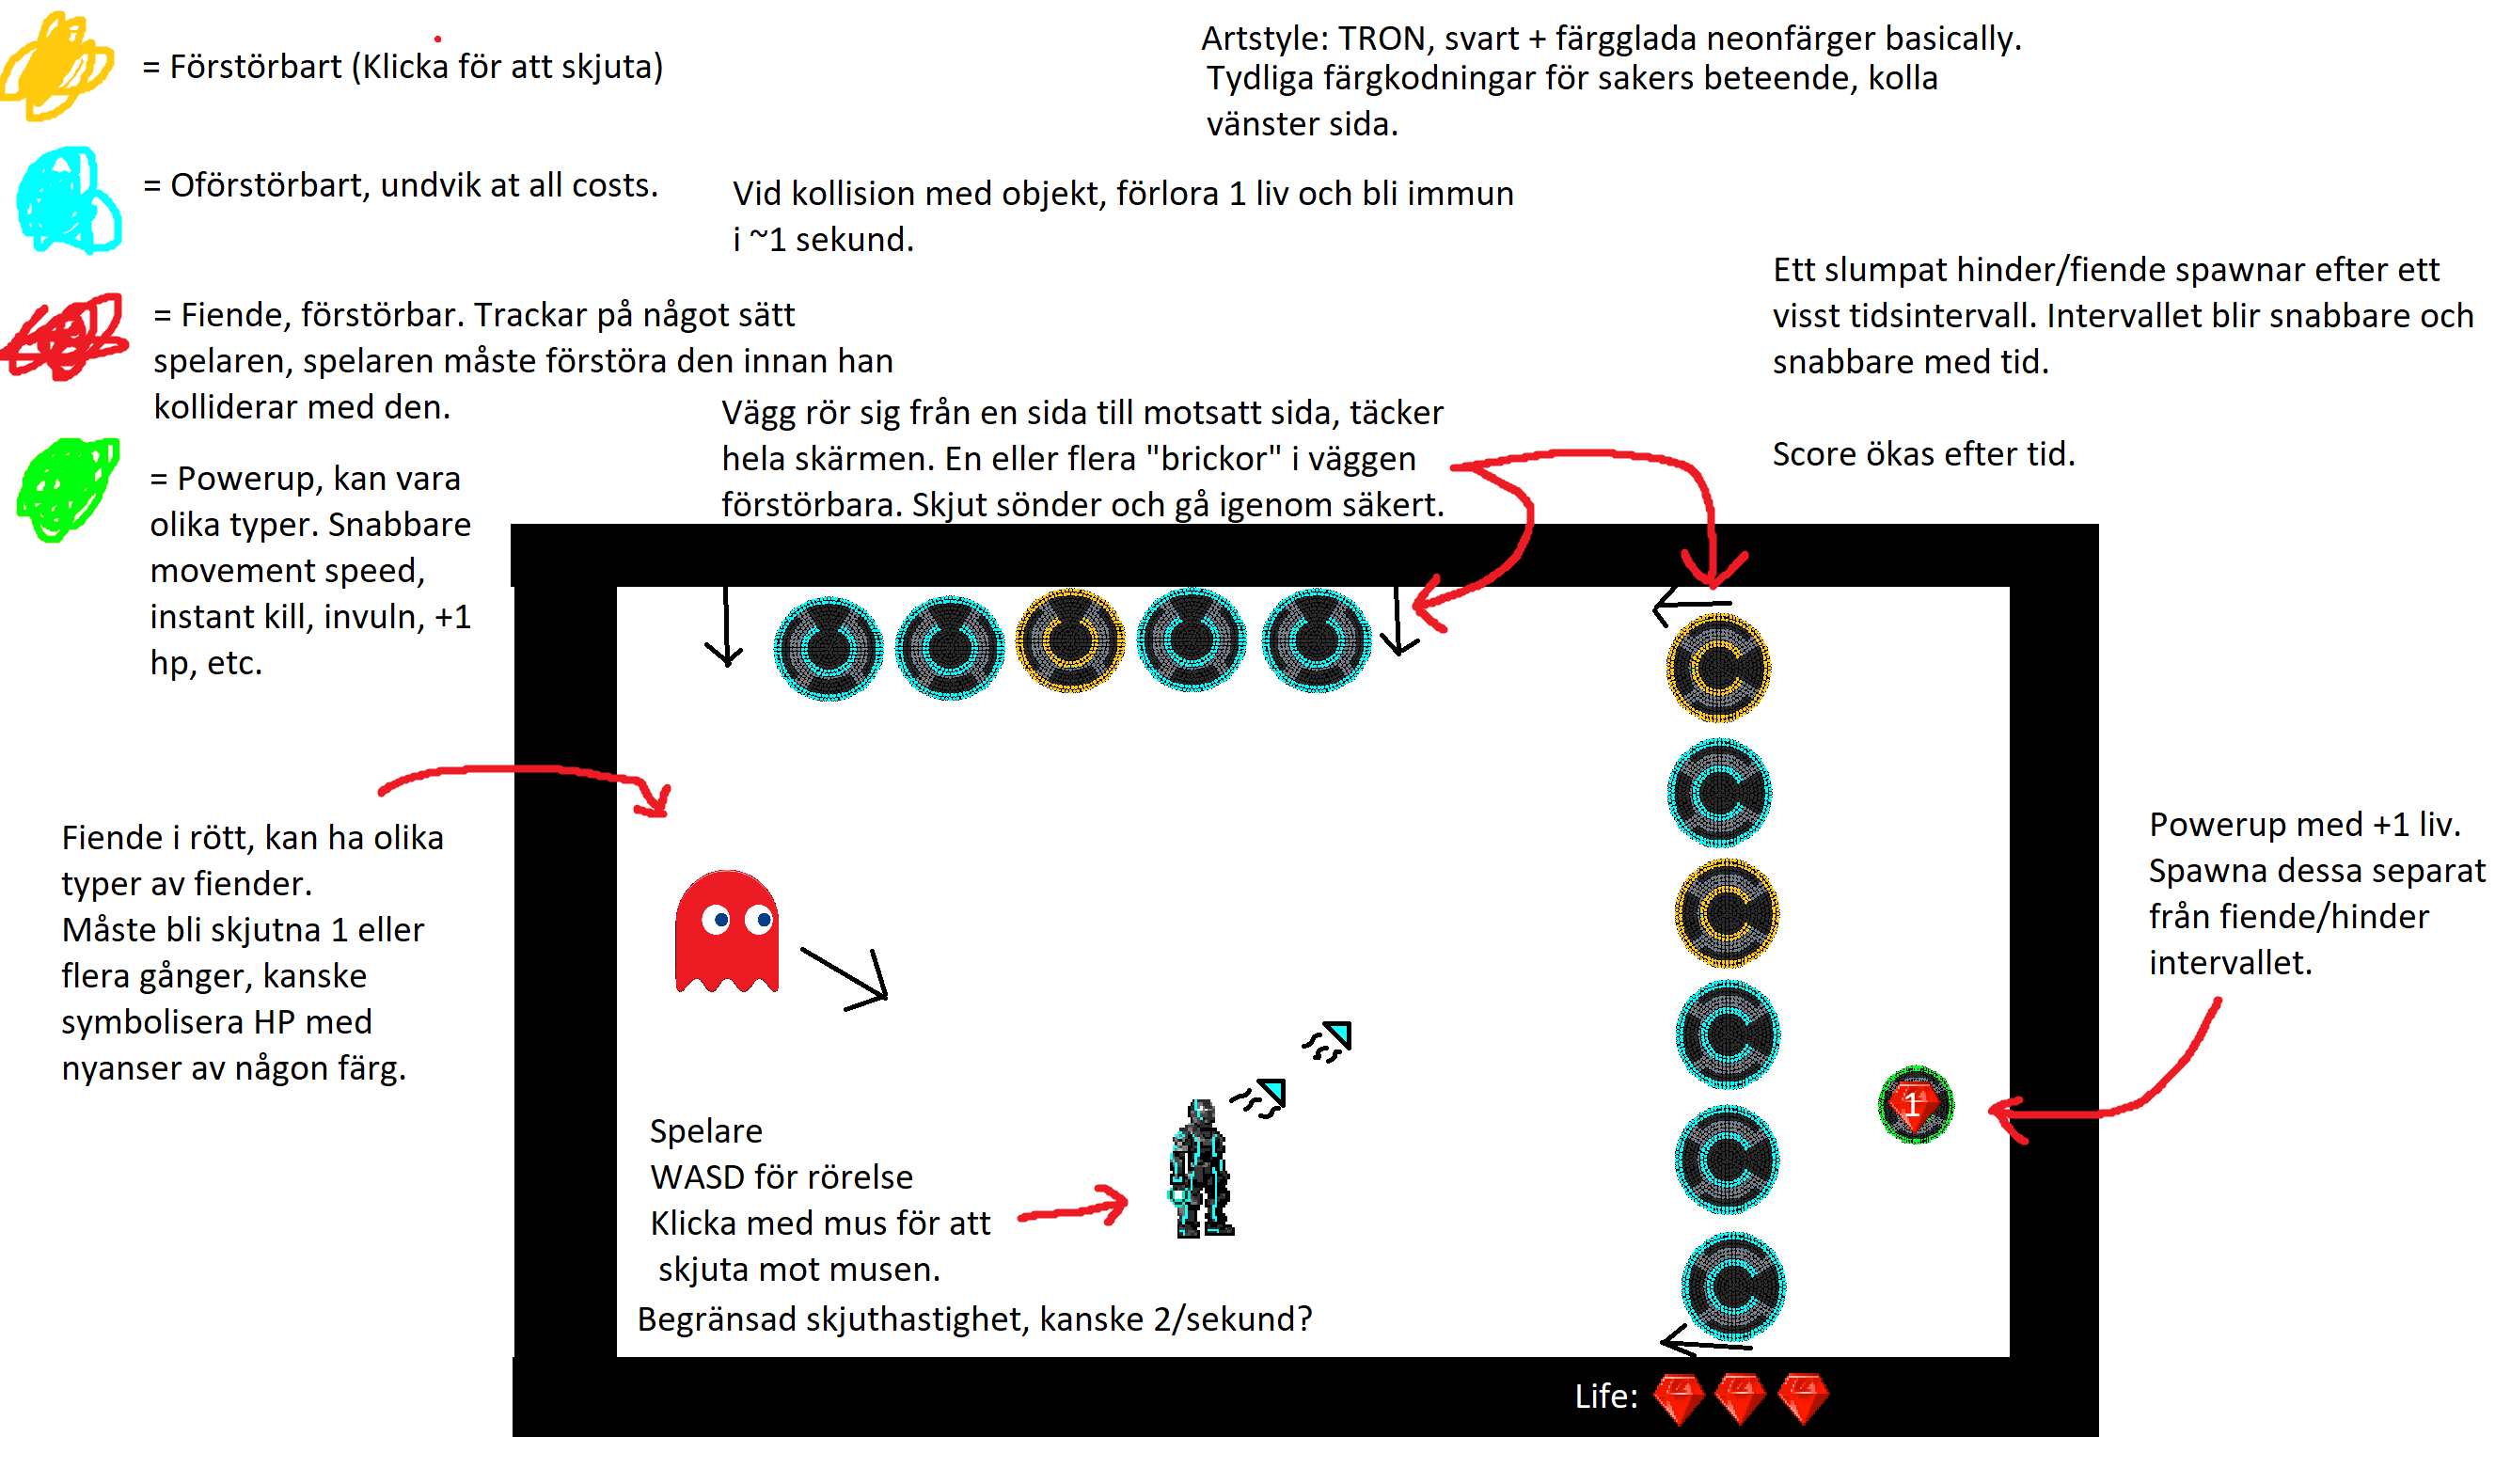
\includegraphics[height=10cm]{sketch.png}

\section{Kravformulering}
\subsection{Ska-krav}

\begin{table}[!h]
\begin{tabularx}{\linewidth}{|l|X|}
\hline
Krav no. & Krav \\\hline

1.1 &  Spelet skall vara tvådimensionellt med synperspektivet ovanifrån.\\\hline

1.2 &  Det skall finnas en spelare.\\\hline

1.2.1 &  Man skall kunna sikta och skjuta (från spelaren) med muspekaren.\\\hline

1.2.2 &  Man skall kunna styra spelaren med WASD.\\\hline

1.2.3 &  Spelaren skall ha liv.\\\hline

1.3.1 &  Det skall finnas fiender.\\\hline

1.3.1.1 &  Fiender skall röra sig mot spelaren.\\\hline

1.3.1.2 &  Vid kollision mellan spelare och fiende skall fiendeobjektet tas bort och skada appliceras på spelaren (Ett liv tas bort).\\\hline

1.3.2 &  Det skall finnas hinder.\\\hline

1.3.2.1 &  Hinder skall röra sig mot andra sidan av världen.\\\hline

1.3.2.2 &  Vid kollision mellan spelare och hinder skall hinderobjektet tas bort och skada appliceras på spelaren. (Ett liv tas bort).\\\hline

1.4 &  Det skall finnas upplockbara power-ups.\\\hline

1.4.1 &  Vid kollision av spelare \& power-up tas power-up ojektet bort.\\\hline

1.4.2 &  Vid kollision av spelare \& power-up appliceras en slumpmässig effekt. (Effekter listade nedan)\\\hline

1.4.2.1 &  Ökad rörelsehastiget under tidsbegränsning.\\\hline
1.4.2.2 &  Instakill (spelarens attack förstör fiender och hinder på ett skott) under tidsbegränsning.\\\hline
1.4.2.3 &  Odödlighet (spelaren ignorerar tagen skada) under tidsbegränsning.\\\hline
1.4.2.4 &  Extra liv, spelaren får ett extra liv (vilka försvinner vid tagen skada och orsakar förlust då inga liv återstår).\\\hline

1.5.1 &  fiender skall dyka upp på ett tidsintervall.\\\hline

1.5.2 &  hinder skall dyka upp på ett tidsintervall.\\\hline

1.6 &  Spelet skall bli svårare med längden enligt sektion 6. Regler\\\hline

1.7 &  Det skall finnas poängräkning baserat på tid.\\\hline

1.8 &  Spelet skall vara konsekvent färgkodat enligt specifikationen för regler.\\\hline

1.9 &  Spelarens livsmängd skall synas i nedre delen av programfönstret.\\\hline

1.10 &  När livsmängden når 0 skall spelet avslutas.\\\hline

1.11 &  Spelaren skall få en period av odödlighet efter att ha tagit skada.\\\hline

1.12 &  Spelet skall utspelas i en arena med begränsade dimensioner.\\\hline

1.13 &  Spelaren skall inte kunna röra sig utanför arenan.\\\hline

\end{tabularx}
\end{table}

\clearpage
\subsection{Bör-krav}

\begin{table}[!h]
\begin{tabularx}{\linewidth}{|l|X|}
\hline
Krav no. & Krav \\\hline
2.1 & Kontrollerna skall vara anpassningsbara. \\\hline

2.2.1 & Det skall finnas variation i typer av fiender. \\\hline

2.2.2 & Det skall finnas variation i typer av power-ups. \\\hline

2.3 & Spelarens high-score skall sparas. \\\hline

2.4 & Fiender och hinder skall, förutom att det kommer fler av dem, bli individuellt starkare med tid. \\\hline

2.5 & Power-ups skall dyka upp på en unik timer. \\\hline

2.6 & Power-ups skall vara kännetecknade av deras utseende. \\\hline

2.7 & Fiender skall symbolisera hur många livspoäng de har kvar. \\\hline

2.8 & Spelet skall ha någon form av ljudeffekter/musik. \\\hline

2.9 & Det skall finnas fina partikeleffekter på ställen där det ser fint ut, men inte för mycket så de blockerar viktig information. \\\hline

\end{tabularx}
\end{table}

\section{Kravuppfyllelse}

\begin{itemize}
    \item Spelet skall simulera en värld som innehåller olika typer av objekt. Objekten skall ha olika beteenden och röra sig i världen och agera på olika sätt när de möter andra objekt.\\
    \\| Krav no. [1.3.X] [1.4.X] [1.5.X] [1.11] [2.2.X] [2.5]\\

    \item Det måste finnas minst tre olika typer av objekt och det skall finnas flera instanser av minst två av dessa. T.ex ett spelarobjekt och många instanser av två olika slags fiendeobjekt.\\
    \\| Krav no. [1.2] [1.3.1] [1.3.2] [1.4] [1.5.X] [2.2.X] [2.4]\\

    \item Ett beteende som måste finnas med är att figurerna skall röra sig över skärmen. Rörelsen kan följa ett mönster och/eller vara slumpmässig. Minst ett objekt, utöver spelaren skall ha någon typ av rörelse.\\
    \\| Krav no. [1.2.2] [1.3.1.1] [1.3.2.1]\\

    \item En figur skall styras av spelaren, antingen med tangentbordet eller med musen. Du kan även göra ett spel där man spelar två stycken genom att dela på tangentbordet (varje spelare använder olika tangenter). Då styr man var sin figur.\\
    \\| Krav no. [1.2.X]\\

    \item Grafiken skall vara tvådimensionell.\\
    \\| Krav no. [1.1]\\

    \item Världen (spelplanen) kan antas vara lika stor som fönstret (du kan göra en större spelplan med scrollning, men det blir lite krångligare).\\
    \\| Krav no. [1.12]\\

    \item Det skall finnas kollisionshantering, det vill säga, det skall hända olika saker när objekten möter varandra, de skall påverka varandra på något sätt. T.ex kan ett av objekten tas bort, eller så kan objekten förvandlas på något sätt, eller så kan ett nytt objekt skapas. (Ett exempel på att skapa/ta bort objekt är när man i Space Invaders trycker på skjuta-knappen, t.ex en musknapp, då avfyras ett laserskott och skottet blir då en ny figur som skapas och placeras i världen, på en position vid laserkanonens mynning. Skottet rör sig framåt (uppåt) och om det träffar ett fiendeskepp tas både skottet och skeppet bort, om skottet kommer utanför spelplanen, dvs det missar, tas det endast bort.)\\
    \\| Krav no. [1.4.1] [1.4.2] [1.3.1.2] [1.3.2.2]\\

    \item Spelet måste upplevas som ett sammanhängande spel som går att spela!\\
    \\| Spelet har bara en värld med enkla kontroller, sammanhängandet kommer handla mycket om vilken grafik som implementeras (Vilket står beskrivet under sektion 7. Visualisering). Utöver detta bör hinder implementeras på så vis att spelaren aldrig skall tvingas ta skada (givet att spelarens förmågor är höga
     och reaktioner är snabba). \\
\end{itemize}

\end{document}
